\documentclass[tikz,border=2pt]{standalone}
\usepackage{amsmath,amssymb}
\usepackage{pgfplots}
\pgfplotsset{compat=1.18}

\begin{document}
% The distribution of X is the rule B -> P(X in B) on the real line: for a continuous X it is
% read off as areas under the density, for any set B (an interval here).
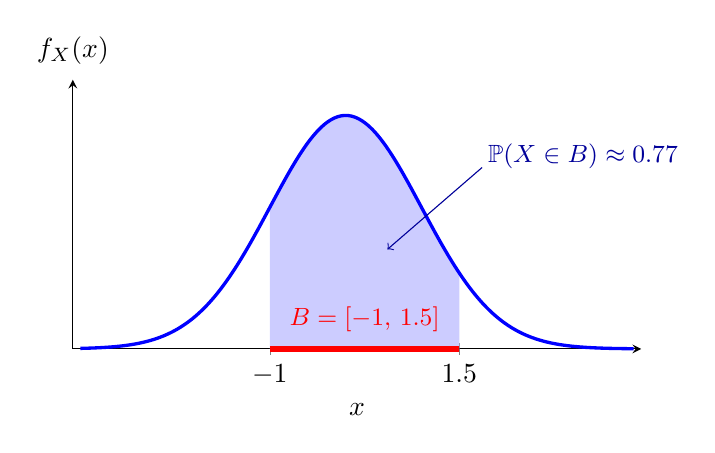
\begin{tikzpicture}
	\begin{axis}[
		axis lines=left, xmin=-3.6, xmax=3.9, ymin=0, ymax=0.46,
		xtick={-1,1.5}, xticklabels={$-1$,$1.5$}, ytick=\empty,
		xlabel={$x$}, ylabel={$f_X(x)$}, ylabel style={rotate=-90, anchor=south, at={(axis description cs:0,1.02)}},
		samples=160, smooth, width=8.8cm, height=5cm, clip=false
		]
		\addplot[fill=blue!20, draw=none, domain=-1:1.5] {exp(-x^2/2)/sqrt(2*pi)} \closedcycle;
		\addplot[blue, very thick, domain=-3.5:3.8] {exp(-x^2/2)/sqrt(2*pi)};
		\draw[red, line width=2pt] (axis cs:-1,0) -- (axis cs:1.5,0);
		\node[red, anchor=south, font=\small] at (axis cs:0.25,0.012) {$B=[-1,\,1.5]$};
		\node[blue!60!black, font=\small, anchor=west] at (axis cs:1.75,0.33) {$\mathbb{P}(X\in B)\approx0.77$};
		\draw[blue!60!black, ->] (axis cs:1.8,0.31) -- (axis cs:0.55,0.17);
	\end{axis}
	
\end{tikzpicture}
\end{document}
